%!TEX root = ../../Main.tex
\graphicspath{{Chapters/Struktur/}}
%-------------------------------------------------------------------------------

\section{TFT Display Module}
TFT Display modulets primære opgave er både at fungere som visuel grænseflade til brugeren, samt at fungere som et slags kontrol modul for hele systemet. Kontrol modul forstået på den måde, at når bruger trykker på knappen på boardet vil det trigger et interrupt, som henter data fra Color Sensor Modulet, optæller den hentede information og displayer det for brugeren.\\ Dette modul afsnit vil beskrive TFT Display modulets funktionalitet, samt overvejelser omkring analyse og design både hardware, softwaremæssigt. I dette afsnit vil kommunikationen mellem TFT Display modulet og resten af systemet også blive beskrevet. 

\subsection{Hardware}
I arkitekturfasen gik den første overvejelse på hvilket display vi skulle benytte som grænsefladen til brugeren. Vi ønskede et displayet som kunne vise farver og havde en nogenlunde opløsning for give en god visuel oplevelse for brugeren. Da vi først havde opsat kravene for vores display, var selve valget ikke særligt svært. I undervisningen har vi arbejdet med ”Graphic TFT Display” fra lektion 4, dette display opfyldte vores ønskede krav angående opløsning samt muligheden for at vise farver. Derfor faldt valgt ret hurtigt på dette display, da det også spillede sammen med vores Arduino 2560. For at kunne påmontere ”Graphic TFT Display” på Arduino Mega 2560, har vi benyttet os af ”ITDB02 Arduino MEGA shield 2.0”. Databladet for dette shield kan læses mere om her i bliagene\cite{man:ITDB02}. I dette datablad er det også markeret hvilke porte ITDB02 shieldet der hører til indgange på displayet.

\subsection{Software}
I og med at dette moduls primære opgave er at være visuel grænseflade for brugeren, har langt det meste arbejde med dette modul lagt i softwaren. 
Hvis man kigger på Graphic TFT Display, kan den fungere i fire forskellige MCU-Interface modes, hvilket simpelt betyder, hvor stor en bus-interface man ønsker at arbejde med. Vi har valgt at arbejde med 16-bit bus-interface, hvordan vi sætter dette, bliver også beskrevet i dette afsnit. 

\begin{figure}[H]
	\centering
	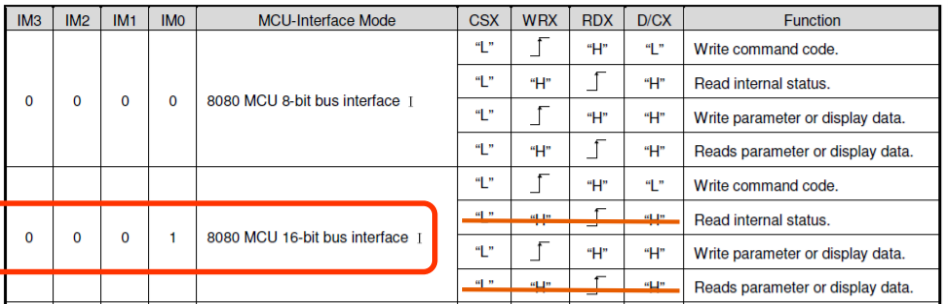
\includegraphics[width = 400pt]{Img/MCU-Interface_Mode.png}
	\caption{MCU-Interface Mode}
	\label{fig:MCU-Interface_Mode}
\end{figure}

I og med at vi udelukkende ønsker at skrive til vores display, vælger vi at ignorere læse kommandoerne, altså retur beskederne som displayet kan give, og udelukkende fokusere på skrive kommandoerne. Derfor er RDX altid sat høj.
Først implementerede vi WriteCommand i vores kode som ses nedenfor.


\begin{lstlisting}
void WriteCommand(unsigned int command)
{
	DATA_PORT_LOW = command;

	DC_PORT &= ~(1<<DC_BIT);
	CS_PORT &= ~(1<<CS_BIT);
	WR_PORT &= ~(1<<WR_BIT);
	
	_NOP();
	WR_PORT |= (1<<WR_BIT);
	_NOP();
}

\end{lstlisting}


Som det ses på figur \autoref{fig:MCU-Interface_Mode} fra databadet\cite{man:ILI9341} side 27, skal DCX og CSX sættes lavt, samt trigger kommandoen på WRX stigende flanke - derfor sættes WRX lav til at starte med. På \autoref{fig:Timedelays} nedenfor ses et skema over de tidsforsinkelser der opstår, ved forskellige operationer. Her ses det at når WRX sættes lav, opstår der en forsinkelse på min 15ns. Derfor er der indsat en NOP() funktion i koden. "NOP" står for ”No Operation”, som vil sige at programmet laver ingenting i en cyklus. Med en MCPU frekvens på 16Mhz svare det til 62,5ns. Herefter sættes WRX høj igen for at trigger kommandoen efterfulgt af endnu en NOP() funktion, da der opstår samme forsinkelse når WRX sættes høj.

\begin{figure}[H]
	\centering
	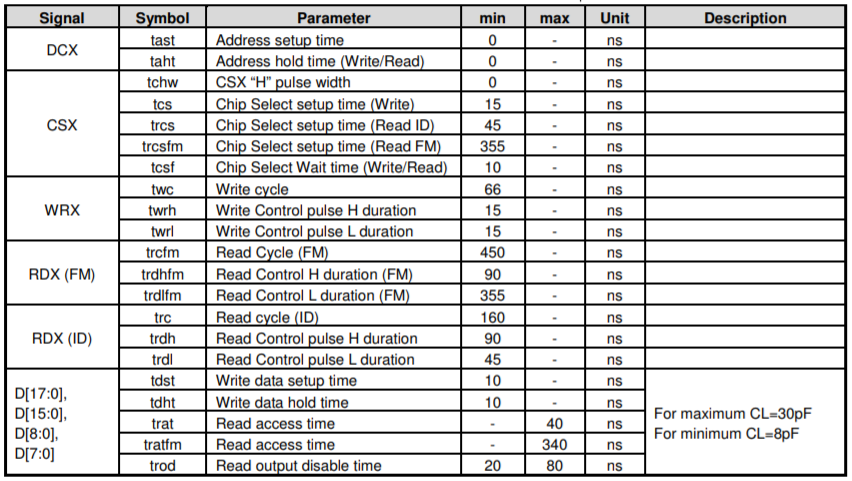
\includegraphics[width = 450pt]{Img/Timedelays.png}
	\caption{Tidsforsinkelser}
	\label{fig:Timedelays}
\end{figure}


Dernæst implementerede vi WriteData, som tilnærmelsesvis ligner WriteCommand bortset fra at DCX skal sættes høj i stedet for lav. Koden for WriteData ses lige nedenfor. Data bliver bitshiftet 8 gang på linje 3, da kun er de 8 LSB der bliver aflæst. På samme måde som WriteCommand trigger WriteData på en stigende flanke på WRX, derfor sættes WRX først lav og dernæst høj, med indsat NOP() funktioner for at tage højde for tidsforsinkelser. 

\begin{lstlisting}
void WriteData(unsigned int data)
{
	DATA_PORT_HIGH = data >> 8;
	DATA_PORT_LOW = data;

	DC_PORT |= (1<<DC_BIT);
	CS_PORT &= ~(1<<CS_BIT);
	WR_PORT &= ~(1<<WR_BIT);

	_NOP();
	WR_PORT |= (1<<WR_BIT);
	_NOP();
}
\end{lstlisting}


I vores DisplayInit() som vi kalder en gang i koden til at Initialisere displayet, koden ses lige nedenfor. Først sættes vores Control Pins som outputs og høje. Port D bit 3 bliver sat lavt, så den er klar til at læse, når brugeren trykker på interrupt-knappen. Dernæst bliver RST sat lav i 300ms, det skyldes at der i databladet\cite{man:ILI9341} på side 230 står minimum 120ms, så det er sat til 300ms for at være på den sikre side. Efter vi igen sætter RST høj, skal vi igen vente 120ms før vi må kalde SleepOut Command. Derfor indsættes et delay på 130ms. Herefter vækkes displayet med Sleepout() kommandoen efterfulgt af Displayon(). Begge disse kommandoer er at finde i databladet\cite{man:ILI9341} på side 83. Den kommando der bliver sendt til MemoryAccessControl() sørger for at sætte rækkefølgen til BGR i stedet for RGB. Til sidst bliver en kommando sendt til InterfacePixelFormat(), denne kommando fortæller displayet at vi ønsker at køre med 16bit pr. pixel se side 134 i databladet\cite{man:ILI9341}. 


\begin{lstlisting}
DisplayInit()
{
	DDRG |= 0b00000111;
	DDRD |= 0b10000000;
	DDRD &= 0b11111011;
	DDRA = 0xFF;
	DDRC = 0xFF;
	PORTG |= 0b00000111;
	PORTD |= 0b10000000;
	PORTD &= 0b11111011;
	
	RST_PORT &= ~(1<<RST_BIT);
	_delay_ms(300);

	RST_PORT |= (1<<RST_BIT);
	_delay_ms(130);
	
	SleepOut();

	DisplayOn();

	MemoryAccessControl(0b00001000);
	
	InterfacePixelFormat(0b00000101);
}
\end{lstlisting}


Efter at have initialiseret og opsat displayet efter eget ønske. Var den næste opgave at kunne skrive tal og bogstaver ud på vores display. Til dette benyttede vi os af et program ved navn ’TheDotFactory’. Vi fik programmet til at udskrive et kæmpe array, som indeholder alle symboler, tal samt bogstaver vi kunne have brug for. Sammen med et tilhørende array, der fortæller længden af hvert symbol samt dens offset. Disse to arrays genereret af programmet ’TheDotFactory’ har vi lagt ind i en h-fil ved navn ”DotFactory.h”.
På den efterfølgende \autoref{TFTDisplayFunktioner} vil funktionerne vi har benyttet blive overordnet blive beskrevet, i vores vedlagte kode vil en mere detaljeret gennemgang af koden kunne ses, i form af kommentar til hver linje kode i den vedlagte kode. 


\begin{table}[]
	\centering
	\caption{Funktioner benyttet til TFT Display}
	\label{TFTDisplayFunktioner}
	\begin{tabular}{|l|l|}
		\hline
		\textbf{Navn}         & \textbf{Beskrivelse}                                                                                                                                                              \\ \hline
		WritePixel() & \begin{tabular}[c]{@{}l@{}}Formålet er at bestemme farven for en pixel. Tager imod 3 parameter.\\ Rød 0-31, grøn 0-63, blå 0-31 smider dem ind i write data.\end{tabular} \\ \hline
		SetColomnAddress() & \begin{tabular}[c]{@{}l@{}}Formålet er at kunne skrive til en hel linje lodret på en gang.\\ Tager imod to parameter start og stop.\end{tabular}                                                                                                                                                                         \\ \hline
		SetPageAddress() & \begin{tabular}[c]{@{}l@{}} Formålet er at kunne skrive til en hel linje vandret på en gang.\\ Tager imod to parameter start og stop. \end{tabular}                                                                                                                                                                        \\ \hline
		FillRectangle() & \begin{tabular}[c]{@{}l@{}} Meningen er at fylde et rektangel med én farve.\\ Tager imod syv parametre: start-x, start-y, bredde, højde,\\ rød, blå og grøn.  \end{tabular}  \\ \hline
		getSymbolParameters() &  \begin{tabular}[c]{@{}l@{}} Den tager tre parametre, start x og start y samt længden på det\\ givne symbol. Formået for denne funktion er at opdele alle de\\ nødvendige informationer for et symbol. Så som længen af symbolet\\ i byte, offset i forhold til arrayet fra TheDotFactory, offset i forhold\\ til displayet. Denne information bliver så videregivet til drawSymbol(). \end{tabular}   \\ \hline
		drawSymbol() &  \begin{tabular}[c]{@{}l@{}}Tager information videregivet fra getSymbolParameters(). Finder det\\ givne symbol i arrayet fra TheDotFactory ved hjælp af de videregivet\\ parametre. Herefter gennemgås symbolet bit for bit, og displayet\\ en sort pixel eller hvid pixel alt efter om det er et ’1’ eller ’0’\\ på den givne plads.  \end{tabular}                                                                                                                                                                                         \\ \hline
		writeString() & \begin{tabular}[c]{@{}l@{}} Tager imod en string. Hvorefter den gennemgår denne string symbol\\ for symbol og kalder getSymbolParameters () som videre kalder\\ drawSymbol() på hvert symbol. Med mindre at symbolet er et\\ mellemrum, så plusses x-positionen med seks.  \end{tabular}                                                                                                                                                                                         \\ \hline
		writeInt() &  \begin{tabular}[c]{@{}l@{}} Tager imod en long int. Hvorefter den int bliver lagt over i et array.\\ Og på hver plads i dette array bliver getSymbolParameters kaldt,\\ efter det første tal er detekteret.   \end{tabular}                                                                                                                                                                                         \\ \hline
		\begin{tabular}[c]{@{}l@{}} DrawRed(),\\ DrawGreen(),\\ DrawBlue() \end{tabular}  &  \begin{tabular}[c]{@{}l@{}} Meningen med denne funktion er at vise en søjle i enten farven rød,\\ grøn eller blå alt efter hvilken af disse tre funktioner der bliver kaldt.\\ Over denne søjle skal så skrives et tal, som følger søjlens højde.\\ Funktionerne modtager to int, den første int angiver tallet som skal\\ stå over søjlen, den anden int angiver højden på søjlen. Tallet\\ bliver vist ved hjælp af funktionen writeInt(), og søjlen bliver vist ved\\ hjælp af funktionen FillRectangle(). Den eneste forskel på disse tre\\ funktioner er farven af søjlen.  \end{tabular} \\ \hline
		drawTotal() &  \begin{tabular}[c]{@{}l@{}} Meningen med denne funktion er at den skal tage tre parametre som\\ antallet af hver farve detekteret. Disse tre parametre bliver så lagt\\ sammen i en totalCount variable, og udregnet hvor stor en procentdel\\ de hver udgør at det samlet antal optællinger. Den procentdel\\ udgør så hvor høj hver enkel søjle skal være. Så vil DrawRed(),\\ DrawGreen() og DrawBlue() blive kaldt hvor de tre parametre vil\\ være tallene over søjlerne, højden vil være den udregnede\\ procentdel og totalCount vil blive vist i øverste højre hjørne\\ ved hjælp af writeInt().  \end{tabular}                                                                                                                                                                                         \\ \hline
	\end{tabular}
\end{table}
\newpage



På \autoref{fig:Flowchart_TFTDisplay_SW} ses et lille flow chart over main koden til TFT Display Modul. Modulet bliver trigget af at brugeren trykker på knappen. Det får modulet til at hente sit input igennem en I2C forbindelse fra Color Sensor Module, som vil blive mere uddybet i det efterfølgende afsnit. Det input bliver så undersøgt, og alt efter hvilket char 'R', 'G' eller 'B' der bliver modtaget optælles den tilhørende conut til den farve, hvorefter displayet bliver clearet og det nye resultat bliver vist. Så er modulet klar til et nyt input.
\begin{figure}[H]
	\centering
	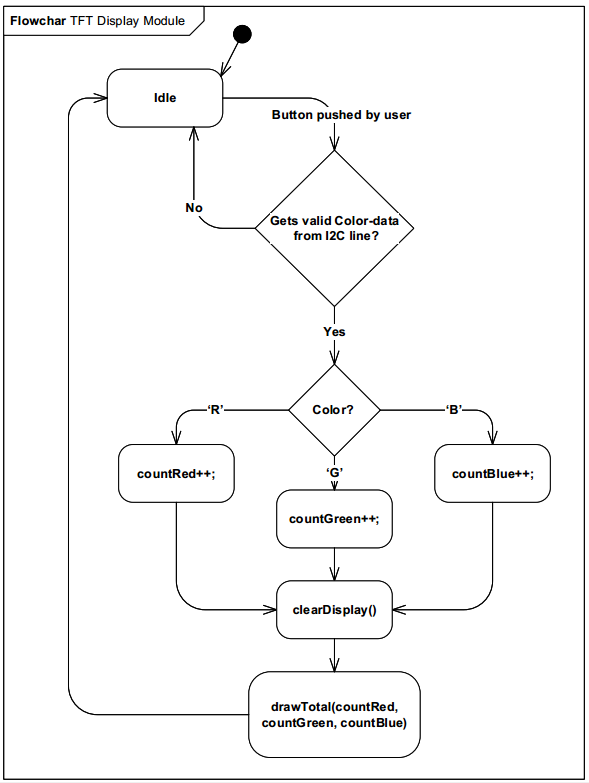
\includegraphics[width = 300pt]{Img/Flowchart_TFTDisplay_SW.png}
	\caption{Flowchart TFT Display software}
	\label{fig:Flowchart_TFTDisplay_SW}
\end{figure}


\subsection{Test}
Efter modulet stod færdig blev en enhedstest af modulet lavet resultatet af dette ses på \autoref{fig:TFT_Display_Module_test}. I testen blev countBlue og countGreen hver plusset op 1 og countRed blev pludset op med 2 en gang i sekundet. Som det kan ses passer vores procentvise fordeling af søjlerne. Blå og grøn søjle har samme højde og den røde søjle er dobbelt så høj. Det er kun i enhedstesten af vi plusser count variablerne op en gang i sekundet. I det færdige system vil denne data komme fra I2C linjen. 


\begin{figure}[H]
	\centering
	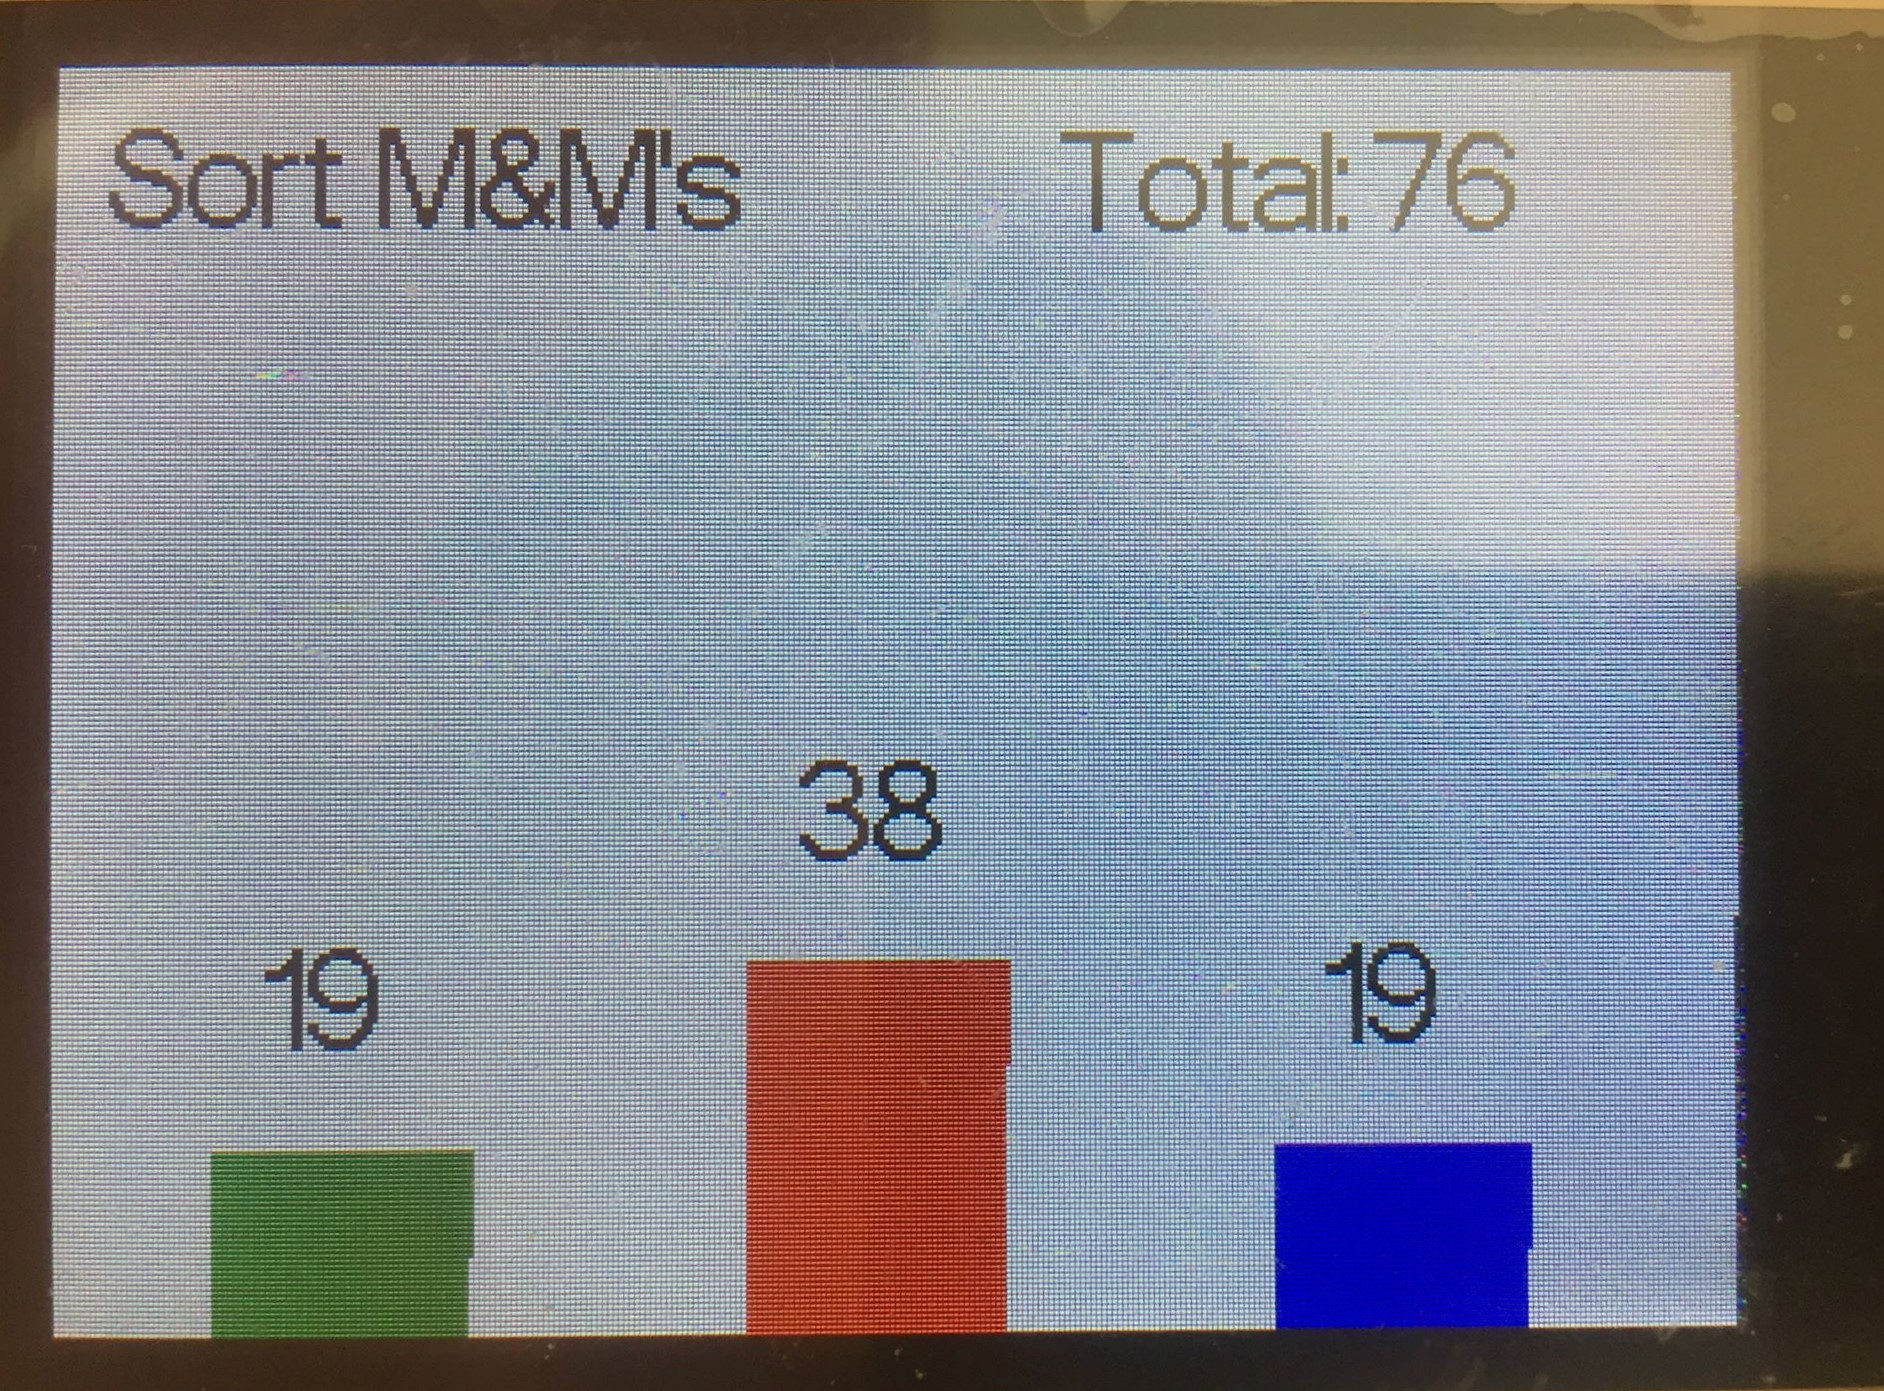
\includegraphics[width = 300pt]{Img/TFT_Display_Module_test.jpg}
	\caption{TFT Display Module enhedstest}
	\label{fig:TFT_Display_Module_test}
\end{figure}
